\begin{figure}[H]
\centering
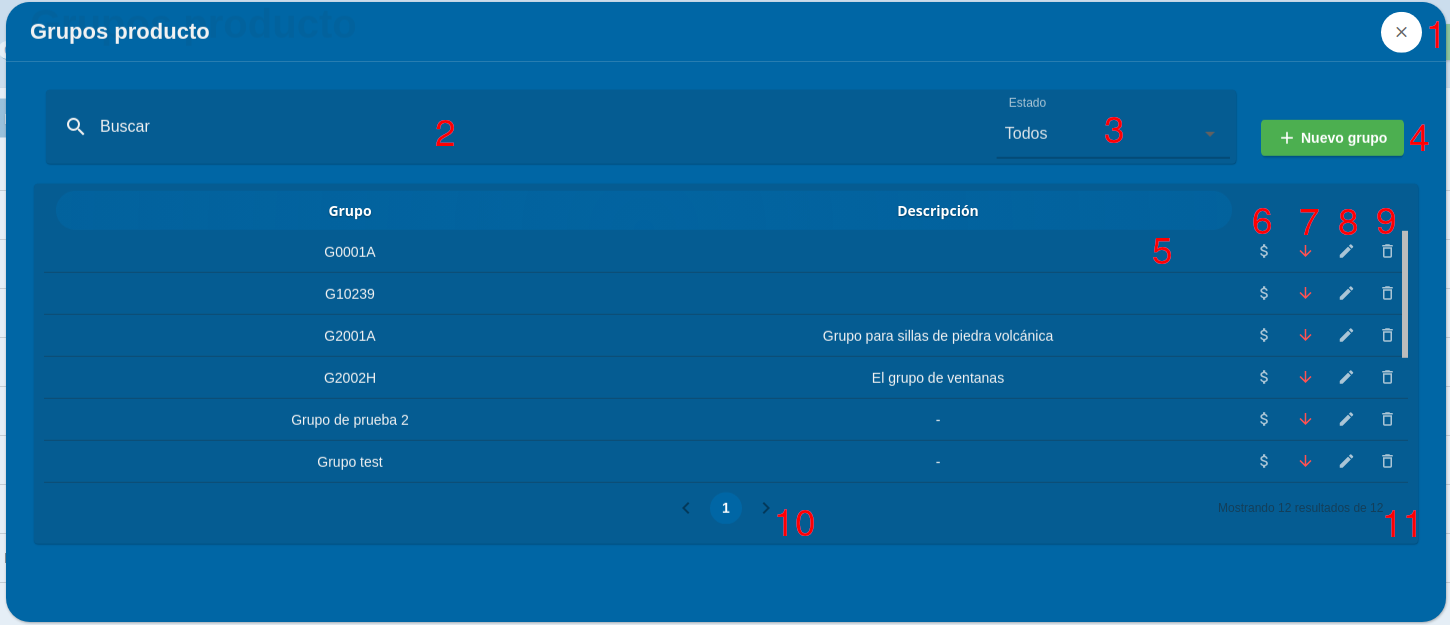
\includegraphics[width=\textwidth,height=\textheight,keepaspectratio]{Escenarios/AD-45-00}
\caption{Escenario - AD-45-00}
\label{fig:AD-45-00}
\end{figure}


Este escenario muestra toda la información referida a los grupos de productos, junto con las acciones disponibles.
El botón \textbf{AD-45-01} permite cerrar la ventana volviendo al escenario \textbf{AD-42-00}. El campo \textbf{AD-45-02} permite ingresar un texto para filtrar los grupos de productos por nombre y la lista desplegable \textbf{AD-45-03} permite al usuario filtrar por los estados en los cuales puede encontrarse el grupo de producto. El botón \textbf{AD-45-04} permite al usuario crear un nuevo grupo de producto y navega al escenario \textbf{AD-46-00}.
El campo \textbf{AD-45-05} muestra la información relacionada a los grupos de productos especificando el nombre y descripción del mismo. El botón \textbf{AD-45-06} permite navegar al escenario \textbf{AD-47-00} para modificar los precios de los productos que pertenecen al grupo indicado, el botón \textbf{AD-48-07} permite al usuario dar de alta/baja un grupo de productos, el botón \textbf{AD-45-08} permite al usuario editar el grupo de producto navegando al escenario \textbf{AD-46-00} y el botón \textbf{AD-45-18} permite al usuario borrar el grupo de producto. 
En \textbf{AD-45-10} se mostrarán las páginas de resultado, pudiendo cambiar de página. En \textbf{AD-45-11} se mostrará cuantos resultados se están visualizando y el total.

\clearpage
